\chapter{Umfrage}



% Introduction Umfrage
Als Ergänzung zur Datenerfassung der GitHub Projekte wurde auch eine Umfrage durchgeführt.
Ziel der Umfrage war es herauszufinden worauf die Nutzer von Open Source achten, wenn sie ein Projekt
wählen. Das übergeordnete Ziel war es die Hypothesen H3, H6 und H8 zu prüfen.
An der Online-Umfrage haben Softwareentwickler der adesso SE, sowie Studenten der TH Rosenheim teilgenommen.
Insgesamt erhielt die Umfrage 308 Antworten. Zur Erstellung der Umfrage wurde \textit{cryptpad.org} 
verwendet \cite{Cryptpad_org}.

Hierbei sollten die Teilnehmer Aussagen zu den Themen Dokumentation, Beliebtheit, Sponsoren und
Entwicklung bewerten. Als Bewertungsskala wurde eine 5-Punkte Likert-Skala verwendet \cite{likertScale}.


% \xo{Interpretation der Durchschnitte: 1 = der Teilnehmende stimmt der Aussage gar nicht zu, 5 =
%     der Teilnehmende stimmt der Aussage vollkommend zu. 3 = Undecided, doesnt matter etc.}



% Dokumentation
\section{Dokumentation}

% Was mussten die Teilnehmer machen?
Im ersten Teil der Umfrage mussten die Teilnehmenden zu zwei Aussagen verschiedene Kriterien bewerten.
Diese Kriterien wurden gewählt basierend auf Erfahrung als Entwickler als auch Beobachtungen vieler
Dokumentationen während der manuellen Datenerfassung zu aus Kapitel
\ref{ssec:manuelle_datenerfassung_dokumentation}.


\bigskip
\noindent
Die erste Aussage war \textit{"Wie wichtig sind Ihnen folgende Aspekte der OSS-Dokumentation"}, mit den Punkten:
\begin{multicols}{2}
    \begin{itemize}
        \setlength\itemsep{0em}
        \item Übersichtlichkeit
        \item Einfache Sprache
        \item Live-Demos
        \item Übersetzungen (z.B. Englisch -> Deutsch)
        \item Das Vorhandsein einer Getting Started Page
        \item Code Beispiele
        \item Strukturierung der Dokumentation
        \item []
    \end{itemize}
\end{multicols}

\bigskip
\noindent
Die zweite Aussage war \textit{"Die folgenden Punkte würden mich von der Nutzung eines OSS-Projekts
    abhalten oder mich möglicherweise dazu veranlassen, nach Alternativen zu suchen."}, mit den Punkten:

\begin{multicols}{2}
    \begin{itemize}
        \setlength\itemsep{0em}
        \item Keine Code Beispiele
        \item Schlecht strukturierte Dokumentation
        \item Dokumentation zu komplex
        \item Fehlende Übersetzung (z.B. fehlende deutsche Übersetzung)
        \item Fehlende Getting Started Page
    \end{itemize}
\end{multicols}



\bigskip
\noindent
% More Detail
Die Aussagen wurden auf einer 5-Punkte Skala bewertet, hierbei entspricht 1 \textit{Stimme gar nicht zu}
und 5 \textit{Stimme vollkommen zu}. Um die Aussagen miteinander zu vergleichen, wurde jeweils der
Mittelwert berechnet.

% Conclusion
Die zwei wichtigsten Aspekte einer Guten Dokumentation sind laut den Befragten, Code Beispiele und
Übersichtlichkeit in beiden Fällen mit einem durchschnittlichen Wert von 4,36. Gefolgt von guter 
Struktur (4,09) und
das Vorhandensein eines \textit{Getting Started} (3,98). Einfache Sprache (3,08) und Live-Demos spielt für
die Befragten eine weniger wichtige Rolle. 
Übersetzungen belegen mit 1,53 den letzten Platz und spielt somit die unwichtigste Rolle in einer 
guten Dokumentation. 


Die zweite Aussage war \textit{"Die folgenden Punkte würden mich von der Nutzung eines OSS-Projekts
    abhalten oder mich möglicherweise dazu veranlassen, nach Alternativen zu suchen."} Am höchsten bewertet
wurde der Punkt \textit{Fehlende Code Beispiele} (4,07) und ist somit der wichtigste Teil einer guten
Dokumentation, gefolgt von schlechter Struktur (3,91). 
Eine komplexe Dokumentation oder das Fehlen einer Getting Started Seite wurde hierbei als mittelmäßig kritisch 
eingestuft, mit einer durchschnittlichen Bewertung von 3,29 bzw. 3,10. Das Fehlen einer Übersetzung ist mit 1,37
das unwichtigste Kriterium.
In den Abbildungen \ref{abb:GuteDoku_BarChart} und
\ref{abb:SchlechteDoku_BarChart} wird das Meinungsbild der Teilnehmer grafisch dargestellt.

% Interpretation beider Fragen.
Zusammenfassend kann man sagen, dass Code Beispiele ein Must Have einer Dokumentation ist.
Das Vorhandensein wird als wichtig eingestuft, während das Fehlen dazu führen könnte, dass Nutzer
zu alternativen greifen würden. Übersetzungen hingegen werden als gleichgültig betrachtet, das
Vorhandensein bietet wenig Mehrwert, die Abwesenheit wird nicht als kritisch betrachtet.

% ---------------------------------------------------- %
% Likert to Kano (kinda)
% https://www.eric-klopp.de/texte/die-kano-methode.php
% ---------------------------------------------------- %


% ----------------------------------------- FreitextFeld ----------------------------------------- %
\bigskip
\noindent
Beide Fragen hatten jeweils ein Freitextfeld, indem die Teilnehmenden die Möglichkeit hatten weitere
Aspekte einer guten bzw. schlechten Dokumentation zu nennen. Diese Freitextfelder waren optional und
wurden von 95 bzw. 71 der gesamten 308 Teilnehmenden genutzt.
Alle Einträge wurden kategorisiert und zusammengefasst.

% Most Used Words
In der Tabelle \ref{tab:freitext_felder_ergebnisse} finden sich die am häufigsten genannten
Punkte. Aktualität, Vollständigkeit und UX waren die am meisten genannten Eigenschaften
bezüglich guter Dokumentation, die jeweiligen Pendants, veraltete Dokumentation, unvollständige
Dokumentation und schlechte UX waren die häufigsten genannten Gründe, um ein OSS Projekt nicht zu
nutzten. Diese drei Merkmale vervollständigen somit die vorhin erwähnten \textit{Must-Haves} einer
guten Dokumentation.

\bigskip
\begin{table}[h]
    \begin{tabular}{lcllc}
        \cline{1-2} \cline{4-5}
        \textbf{Gute Dokumentation} & \multicolumn{1}{l}{\textbf{Erwähnungen}} & \hspace{1cm} & \textbf{Schlechte Dokumentation}   & \multicolumn{1}{l}{\textbf{Erwähnungen}} \\ \cline{1-2} \cline{4-5}
        Aktualität                  & 28                                       &              & Veraltet                           & 25                                       \\
        Vollständigkeit             & 21                                       &              & Unvollständig                      & 15                                       \\
        Gute UX                     & 14                                       &              & Schlechte UX                       & 11                                       \\
        Versionierung               & 10                                       &              & Fehlerhaft                         & 7                                        \\
        Changelog vorhanden         & 6                                        &              & Keine Doku vorhanden               & 6                                        \\
        Gute Code Beispiele         & 5                                        &              & Code Beispiele funktionieren nicht & 5
    \end{tabular}%
    \caption{Häufigste Erwähnungen der Freitexter}
    \label{tab:freitext_felder_ergebnisse}
\end{table}


\subsubsection*{Anmerkung:}
\textit{Im Fall von UX wurden folgende Punkte zusammengefasst: Suchfunktion/Verlinkung, Design und
Übersichtlichkeit.}


\bigskip
\bigskip
\noindent
Die abschließende Frage zum Thema Dokumentation war: \textit{"Hat eine schlechte Dokumentation Sie jemals
    dazu gebracht, ein alternatives Projekt zu wählen?"}. 81\% der Teilnehmen haben diese Frage mit
\textit{"Ja"} beantwortet. 


% Gutes Zitat tbh.
% "Gar keine Dokumentation ist ein Zeichen von fehlendem Engagement/Einsatz - nicht vertrauenswürdig"


% ------------------------------------------ Bar Charts ------------------------------------------ %
\begin{figure}[h]
    \centering
    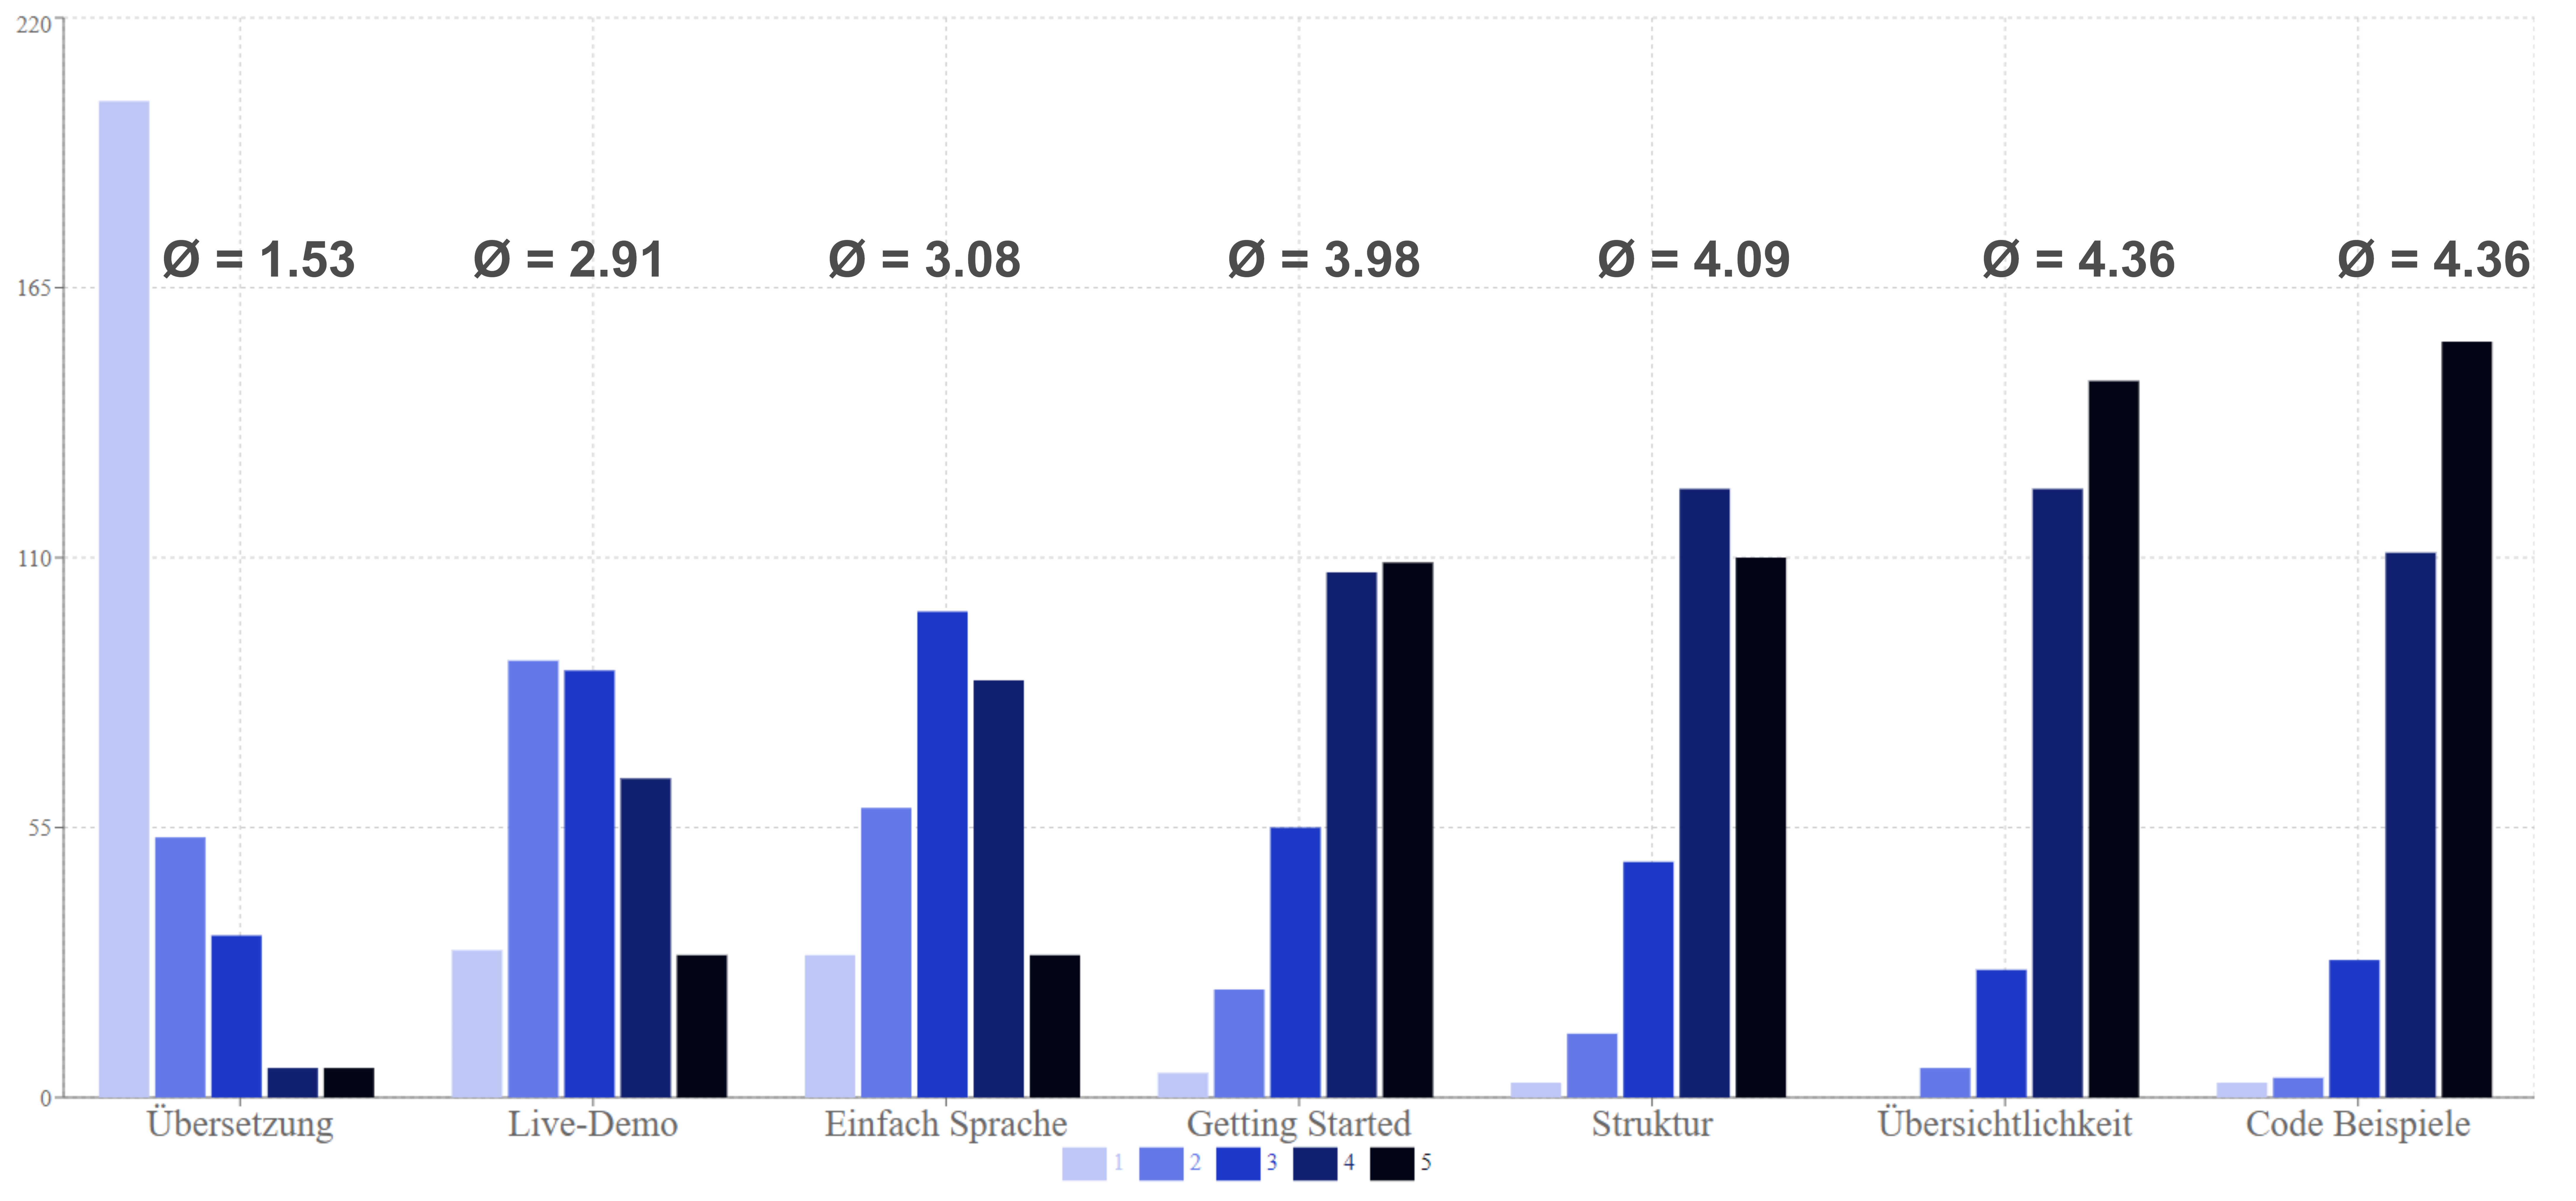
\includegraphics[scale=0.05]{figures/05/GuteDoku_BarChart.png}
    \caption{Antworten: Was zeichnet Gute Dokumentation aus?}
    \label{abb:GuteDoku_BarChart}
\end{figure}

\begin{figure}[h]
    \centering
    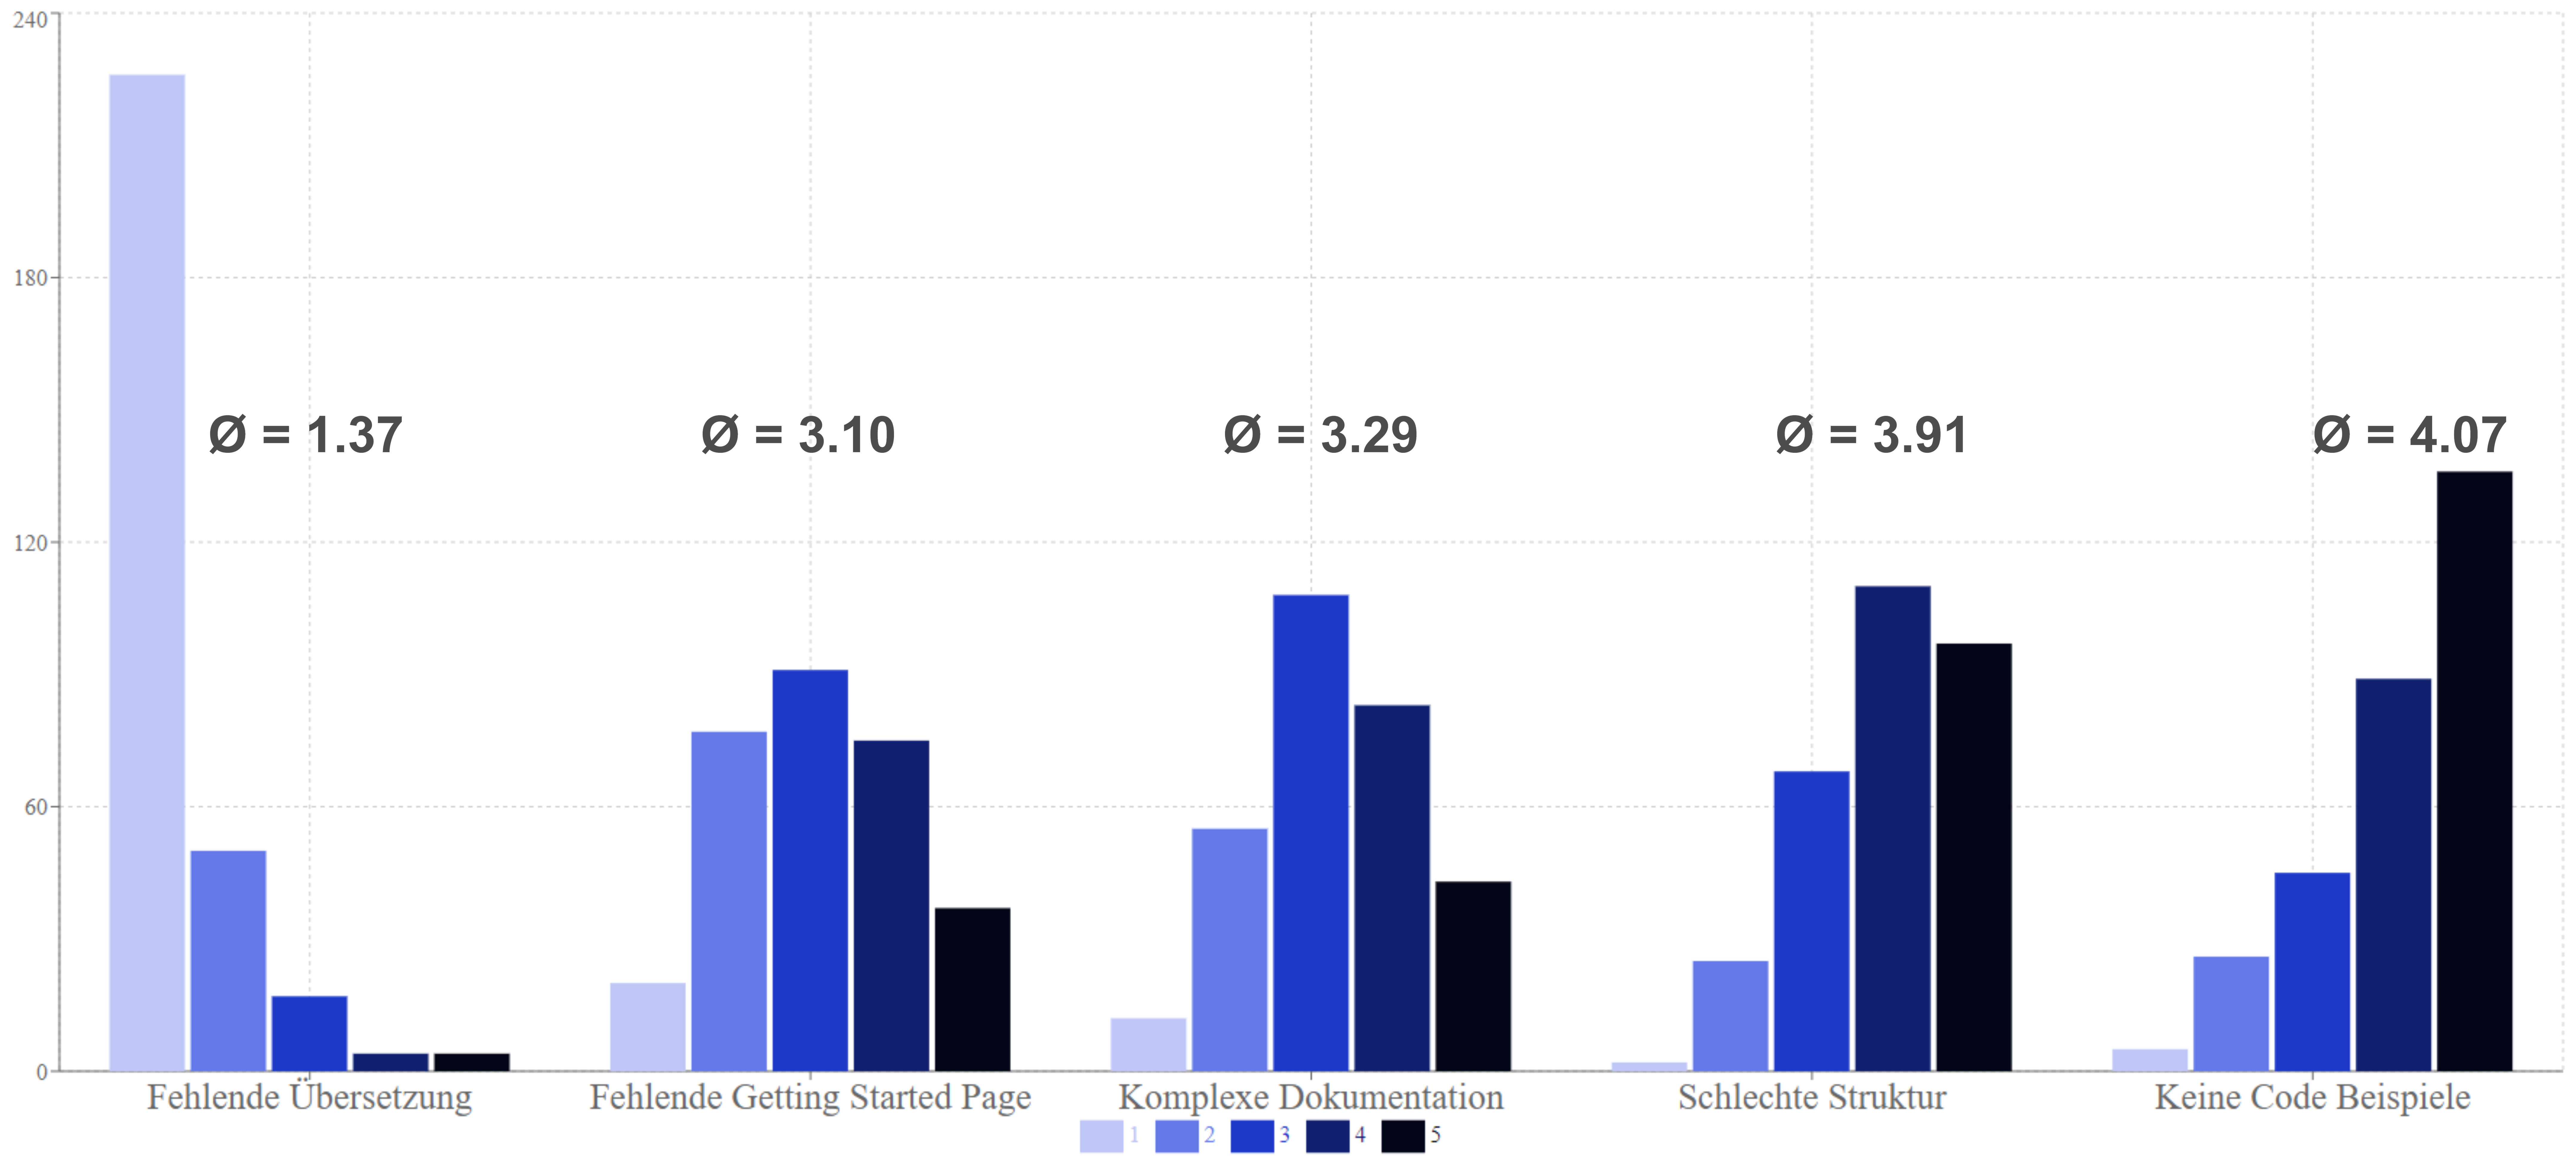
\includegraphics[scale=0.05]{figures/05/SchlechteDoku_BarChart.png}
    \caption{Antworten: Was zeichnet Gute Dokumentation aus?}
    \label{abb:SchlechteDoku_BarChart}
\end{figure}

% Beliebtheit
\newpage
%! newpage
\cleardoublepage %! \cleardoublepage

\section{Beliebtheit}\label{sec:Beliebtheit}
Im zweiten Teil der Umfrage, soll geklärt werden, welchen Einfluss die Beliebtheit, bei der Wahl
eines Projektes hat. Wie zuvor auch sollten die Teilnehmer Kriterien auf einer 5-Punkte Skala bewerten.
Die Mittelwerte der Antworten finden sich in Tabelle \ref{tab:beliebtheit} wieder.

\bigskip
\noindent
Die Aussage war \textit{"Wie sehr achten Sie bei der Auswahl von OSS auf..."}, mit den Punkten:
\begin{multicols}{2}
    \begin{itemize}
        \setlength\itemsep{0em}
        \item Anzahl der GitHub Sterne
        \item Anzahl der Mitwirkenden eines
              Projektes
        \item Anzahl von Sponsoren
        \item Trends
        \item Anzahl an Fragen und Antworten auf\\ StackOverflow
    \end{itemize}
\end{multicols}

\noindent
Diese Punkte wurden gewählt, da es klassischen Vergleichsmerkmalen sind, um die Beliebtheit von OSS
zu vergleichen. GitHub Sterne und Downloads sind eine schnelle und einfache Methode, um die aktuelle 
Beliebtheit eines Projektes zu vergleichen. Trends hingegen stellen GitHub Sterne oder Downloads 
über Zeit dar, häufig genutzte Tools für die Analyse von Trends sind
\textit{StackOverflow Trends}\footnote{\url{https://insights.stackoverflow.com/trends}},
\textit{npm trends}\footnote{\url{https://www.npmtrends.com/}} oder
\textit{Google Trends}\footnote{\url{https://trends.google.de/trends/}}.


% Daten beschreiben
Anders als bei der Dokumentation gibt es hier kein Kriterium mit starker Zustimmung. Die Downloads
sind hierbei mit einer durchschnittlich Zustimmung von 3,27 die beliebtes Vergleichsmetrik für Beliebtheit
gefolgt von Sternen (2,92). Anzahl der Mitwirkenden (2,68), StackOverflow Fragen und Antworten (2,60) sowie 
Trends (2,23) werden tendenziell weniger beachtet. Die Anzahl der Sponsoren wird mit einer durchschnittlichen
Bewertung (1,7) fast gar nicht beachtet. 


Des Weiteren gaben 46\% der Teilnehmer an, dass die geringer Popularität eines Projekts sie schon 
mal davon abgehalten hat dieses zu nutzten.  

% Die leichte Ablehnung der Kriterien deckt sich mit diesem Ergebnissen. Nutzer achten auf Beliebtheit weniger als auf die 
% Qualität der Dokumentation bei der Wahl von OSS.

\begin{table}[h]
    %\resizebox{\textwidth}{!}{%
        \begin{tabular}{cccccc}
            \hline
            Downloads & Sterne & Mitwirkende & StackOverflow Fragen/Antworten & Trends & Sponsoren \\ \hline
            3.27      & 2.92   & 2.68        & 2.60                           & 2.23   & 1.7
        \end{tabular}%
    %}
    \caption{\label{tab:beliebtheit}Einfluss der Beliebtheitsmerkmalen bei der Wahl von OSS}
\end{table}

% Sponsoren
% \newpage
\section{Sponsoren}\label{sec:umfrage_sponsoren}


Im dritten Teil der Umfrage sollte herausgefunden werden, welchen Einfluss Sponsoren bei der OSS Wahl
spielen. Auch hier wurde mit der 5-Punkte Skala bewertet, mit der Frage: \textit{"Bewerten Sie folgende
    Aussagen."} Die Aussagen waren:

\begin{enumerate}
    \setlength\itemsep{0em}
    \item Projekte mit Sponsoren wirken zukunftssicherer
    \item Ich bevorzuge es, wenn möglich, Projekte mit Sponsoren zu nutzten
    \item Gesponserte Projekte sind meistens qualitativ besser
\end{enumerate}

\noindent
Mit einer sehr schwachen Zustimmung von durchschnittlich 3,27 gaben die Teilnehmer an, dass sie 
Projekte mit Sponsoren als zukunftssicherer empfinden. Projekte mit Sponsoren werden tendenziell
weder stark bevorzugt (2,92) noch als qualitativ hochwertiger empfunden (2.68).

\begin{table}[h]
    \begin{tabular}{cccccc}
        \hline
        Aussage: \hspace{1cm} & 1.   & \hspace{0.75cm} & 2.   & \hspace{0.75cm} & 3.   \\ \hline
                              & 3.27 &                 & 2.92 &                 & 2.68
    \end{tabular}%
    \caption{\label{tab:sponsorens}Einfluss von Sponsoren}
\end{table}





% Development
\newpage
\section{Development}
Im vierten Teil der Umfrage ging es um den Einfluss des Entwicklungsprozesses bei der Auswahl von
OSS. Die Frage war: \textit{"Wie sehr achten Sie auf die Folgenden Punkte, wenn Sie ein Projekt
    wählen?"}

\todo{Warum genau diese Punkte?}

\begin{multicols}{2}
    \begin{itemize}
        \setlength\itemsep{0em}
        \item Anzahl aktiver Maintainer
        \item Ticket/Issue Verhältnis Open/Closed
        \item Antwortzeit der Entwickler auf Tickets/Issues
        \item Regelmäßigkeit der Commits
        \item Aktualität des letztes Commit
        \item []
    \end{itemize}
\end{multicols}

\noindent
\todoo{Die gewählten Punkte sind auf GitHub einsehbare Daten, welche als Metriken der Entwicklung
    verwendet werden können.}

\begin{table}[ht]
    %\resizebox{\textwidth}{!}{%
    \begin{tabular}{ccccccc}
        \hline
        Aktualität & Anzahl der Maintainer & Regelmäßigkeit & Verhältnis & Antwortzeit \\ \hline
        3.94       & 3.33                  & 3.28           & 2.90       & 2.86
    \end{tabular}%
    %}
    \caption{\label{tab:development}Einfluss des Entwicklungsprozesses}
\end{table}

\noindent
Ähnlich wie bei der Dokumentation (Sieh Tabellen \ref{tab:freitext_felder_ergebnisse}) legen die Nutzer
einen großen Wert auf Aktualität. \todoo{Gefolgt von Anzahl der Maintainer und Regelmäßigkeit der
    Commits}
Auf Tickets wird hierbei weniger geachtet, weder das Verhältnis zwischen offenen und geschlossen
Tickets noch auf die Antwortzeit der Entwickler auf diese.


\newpage %! new page
\cleardoubleemptypage
\section{Freie Kategorisierung der Erfolgskriterien}\label{sec:umfrage_last_question}


Im letzten Teil der Umfrage sollten die Teilnehmer verschiedene Kriterien per
\textit{Drag and Drop} sortieren. Die Fragestellung lautete
\textit{Sortieren Sie nach den für Sie wichtigsten Kriterien bei der Auswahl von OSS.}
mit folgenden Punkten zum Sortieren


\begin{multicols}{2}
    \begin{itemize}
        \setlength\itemsep{0em}
        \item Gute Dokumentation
        \item Beliebtheit
        \item Anzahl von offenen Issues/Tickets
        \item Trends
        \item Projekt hat Sponsoren
        \item []
    \end{itemize}
\end{multicols}


\noindent
Aufgrund der Übersichtlichkeit hat sich die Auswahl hier auf fünf beschränkt. Es wurde versucht
alle vorherigen Themen abzudecken.
Je nach Platzierung, haben die Kriterien Punkte bekommen, 5 Punkte für den ersten Platz, 4 für den
zweiten usw. der letzte Platz bekam einen Punkt.

Das wichtigste Kriterium ist Gute Dokumentation mit 1329 Punkten, gefolgt von Beliebtheit (1165),
Anzahl der offenen Issues/Tickets (794), Trends (624), Projekt hat Sponsoren (559).
